\documentclass[9pt,aspectratio=169,xcolor=table]{beamer}

%~~~~~~~~~~~~~~~~~~~~~~~~~~~~~~~~~~~~~~~~~~~~~~~~~~~~~~~~~~~~~~~~~~~~~~~~~~~~~~
% Use roboto Font (recommended)
\usepackage[sfdefault]{roboto}
\usepackage[utf8]{inputenc}
\usepackage[T1]{fontenc}
%~~~~~~~~~~~~~~~~~~~~~~~~~~~~~~~~~~~~~~~~~~~~~~~~~~~~~~~~~~~~~~~~~~~~~~~~~~~~~~

%~~~~~~~~~~~~~~~~~~~~~~~~~~~~~~~~~~~~~~~~~~~~~~~~~~~~~~~~~~~~~~~~~~~~~~~~~~~~~~
% Define where theme files are located. ('/styles')
\usepackage{styles/fluxmacros}
\usefolder{styles}
% Use Flux theme v0.1 beta
% Available style: asphalt, blue, red, green, gray
\usetheme[style=gray]{flux}
%~~~~~~~~~~~~~~~~~~~~~~~~~~~~~~~~~~~~~~~~~~~~~~~~~~~~~~~~~~~~~~~~~~~~~~~~~~~~~~

%~~~~~~~~~~~~~~~~~~~~~~~~~~~~~~~~~~~~~~~~~~~~~~~~~~~~~~~~~~~~~~~~~~~~~~~~~~~~~~
% Extra packages
\usepackage{booktabs}
\usepackage{colortbl}
\usepackage{ragged2e}
\usepackage{amssymb}
\usepackage{multirow}
\usepackage{tikz}
\usetikzlibrary{arrows.meta, positioning, fit, backgrounds, calc, decorations.pathreplacing}
\setbeamertemplate{itemize items}[square]
\usepackage[scaled=.92]{beramono}
\usepackage{listings}
\usepackage{styles/lstlangarm}
\usepackage{array}
\definecolor{bgcolor}{HTML}{F2E9E9}
% lstlangarm.sty references \color{mauve} for string literals but never defines
% it -- only fires when a listing contains a string. Define it here.
\definecolor{mauve}{rgb}{0.58,0,0.82}
% lstlangarm's C style sets commentstyle=green!20, which is unreadable on the
% pink listing background. Darken it globally.
\lstset{commentstyle=\color{green!45!black}}
% ragged-right fixed-width column -- must be defined in the preamble, never
% inside a frame (\newcolumntype's #1 breaks beamer's frame scanner)
\newcolumntype{R}[1]{>{\RaggedRight\arraybackslash}p{#1}}
%~~~~~~~~~~~~~~~~~~~~~~~~~~~~~~~~~~~~~~~~~~~~~~~~~~~~~~~~~~~~~~~~~~~~~~~~~~~~~~
% Table striping: odd rows white, even rows very light gray.
% Needs \documentclass[...,xcolor=table]{beamer} (beamer loads xcolor itself,
% so the option must go on the class, not \usepackage).
\definecolor{stripe}{gray}{0.94}
% \striped makes body rows alternate white, gray, white, ... starting white.
% \rowcolors counts from the first coloured body row; the header is not counted.
\newcommand{\striped}{\rowcolors{1}{white}{stripe}}
%~~~~~~~~~~~~~~~~~~~~~~~~~~~~~~~~~~~~~~~~~~~~~~~~~~~~~~~~~~~~~~~~~~~~~~~~~~~~~~

%~~~~~~~~~~~~~~~~~~~~~~~~~~~~~~~~~~~~~~~~~~~~~~~~~~~~~~~~~~~~~~~~~~~~~~~~~~~~~~
% TikZ block styles -- matches ch1/ch2
% Colour variables are named identically in the book's stm32primer.tex, so any
% tikzpicture using only the \tikzset{...} styles below can be copied verbatim
% between slides and book. Only the \definecolor/\colorlet VALUES differ: the
% book is printed, so it keeps every stroke pure black with muted fills. These
% slides are projected, so both fill AND stroke are bright and saturated to
% grab attention -- see stm32primer.tex for the print palette.
\definecolor{blkfill}{HTML}{DCEBFF}
\definecolor{blkline}{HTML}{1565C0}
\definecolor{accentfill}{HTML}{FFE0B2}
\definecolor{accentline}{HTML}{E65100}
\definecolor{memfill}{HTML}{DFF5DA}
\definecolor{memline}{HTML}{2E7D32}
\definecolor{cellfill}{HTML}{FFFFFF}
\definecolor{cellline}{HTML}{424242}
\definecolor{bitmaskfill}{HTML}{DCEBFF}
\definecolor{bitmaskline}{HTML}{1565C0}
\definecolor{bithitfill}{HTML}{FFE0B2}
\definecolor{bithitline}{HTML}{E65100}
\tikzset{
  blk/.style   = {rectangle, rounded corners=2pt, draw=blkline, fill=blkfill,
                  thick, align=center, font=\small, minimum height=9mm, inner sep=3pt},
  cpublk/.style= {rectangle, rounded corners=2pt, draw=accentline, fill=accentfill,
                  thick, align=center, font=\small\bfseries, minimum height=9mm, inner sep=3pt},
  memblk/.style= {rectangle, rounded corners=2pt, draw=memline, fill=memfill,
                  thick, align=center, font=\small, minimum height=9mm, inner sep=3pt},
  cell/.style  = {rectangle, draw=cellline, fill=cellfill, align=center,
                  font=\normalsize\ttfamily, minimum height=7mm, inner sep=2pt},
  lbl/.style   = {font=\scriptsize, text=Gray},
  flow/.style  = {-{Stealth[length=2mm]}, thick, draw=blkline},
  busline/.style={thick, draw=cellline},
  % ---- bit-diagram styles, matching the book's chapter4.tex figures ----
  bitcell/.style={draw=cellline, fill=cellfill, thick,
      minimum width=5.4mm, minimum height=5.4mm, inner sep=0pt,
      font=\scriptsize\ttfamily, anchor=center},
  bitmask/.style={bitcell, fill=bitmaskfill, draw=bitmaskline},
  bithit/.style={bitcell, fill=bithitfill, draw=bithitline,
      font=\scriptsize\ttfamily\bfseries},
  rowlab/.style={font=\scriptsize, text=Gray, anchor=east},
  oplab/.style={font=\scriptsize\itshape, text=Gray, anchor=west},
}
% ---------------------------------------------------------------------------
% Typeset C shift operators in monospace WITHOUT the << >> guillemet ligature.
% Copied from the book's main.tex so the bit-manipulation figures match.
% ---------------------------------------------------------------------------
\newcommand{\shl}{\texttt{<{}<}}
\newcommand{\shr}{\texttt{>{}>}}
\newcommand{\shiftl}[2]{\texttt{#1\,}\shl\texttt{\,#2}}
\newcommand{\shiftx}[3]{\texttt{#1\,}#2\texttt{\,#3}}
% \bitrow{y}{highlight style}{8 comma-separated bit values}{bit to highlight}{row label}
% \bitfieldrow{y}{highlight style}{8 values}{low bit of 2-bit field}{row label}
\newcommand{\bitrow}[5]{%
    \node[rowlab] at (-0.55,#1) {#5};
    \foreach \v [count=\i from 0] in {#3}{
        \pgfmathsetmacro{\bx}{\i*0.62}
        \pgfmathtruncatemacro{\bitnum}{7-\i}
        \ifnum\bitnum=#4
            \node[#2] at (\bx,#1) {\v};
        \else
            \node[bitcell] at (\bx,#1) {\v};
        \fi
    }
}
\newcommand{\bitfieldrow}[5]{%
    \node[rowlab] at (-0.55,#1) {#5};
    \foreach \v [count=\i from 0] in {#3}{
        \pgfmathsetmacro{\bx}{\i*0.62}
        \pgfmathtruncatemacro{\bitnum}{7-\i}
        \pgfmathtruncatemacro{\hi}{#4+1}
        \ifnum\bitnum=#4
            \node[#2] at (\bx,#1) {\v};
        \else\ifnum\bitnum=\hi
            \node[#2] at (\bx,#1) {\v};
        \else
            \node[bitcell] at (\bx,#1) {\v};
        \fi\fi
    }
}
% NOTE (theme quirks -- all fail SILENTLY, always page through the PDF):
%  - a second \\ inside a nested {...} group in a TikZ node breaks parsing
%  - {\small ...} wrapped around a nested itemize eats the frame title + list
%  - \usebeamercolor on a [plain] frame falls through to an unstyled default
%  - \newcolumntype inside a frame breaks beamer's frame scanner
%  - lstlisting needs \begin{frame}[fragile]
%  - a TikZ picture wider than its column silently overflows into neighbours
%~~~~~~~~~~~~~~~~~~~~~~~~~~~~~~~~~~~~~~~~~~~~~~~~~~~~~~~~~~~~~~~~~~~~~~~~~~~~~~

%%%%%%%%%%%%%%%%%%%%%%%%%%%%%%%%%%%
%% BEGIN CONDITIONAL COMPILATION %%
%%%%%%%%%%%%%%%%%%%%%%%%%%%%%%%%%%%
\newif\ifwebex
%\webextrue % uncomment to generate section separator
\ifwebex
\AtBeginSection[]{
  \begin{frame}
  \vfill
  \centering
  \begin{beamercolorbox}[sep=8pt,center,shadow=true,rounded=true]{title}
    \usebeamerfont{title}\insertsectionhead\par%
  \end{beamercolorbox}
  \vfill
  \end{frame}
}
\else
\AtBeginSection[]
{
{
    \setbeamercolor{background canvas}{bg=yellow!10}
    \begin{frame}[plain]
        \frametitle{Table of Contents}
        \tableofcontents[currentsection]
    \end{frame}
}
}
\fi
%%%%%%%%%%%%%%%%%%%%%%%%%%%%%%%%%%%
%% END CONDITIONAL COMPILATION   %%
%%%%%%%%%%%%%%%%%%%%%%%%%%%%%%%%%%%

%~~~~~~~~~~~~~~~~~~~~~~~~~~~~~~~~~~~~~~~~~~~~~~~~~~~~~~~~~~~~~~~~~~~~~~~~~~~~~~
% Information
\title{Embedded C and CMSIS}
\subtitle{\emph{Introduction to ARM Cortex-M Microprocessors} --- Chapter 4}
\author{Mun\'{i}m Zabidi}
\institute{\color{primary}Faculty of Electrical Engineering, Universiti Teknologi Malaysia}
\date{\today}
\titlegraphic{assets/logoutmwhite.png}
%~~~~~~~~~~~~~~~~~~~~~~~~~~~~~~~~~~~~~~~~~~~~~~~~~~~~~~~~~~~~~~~~~~~~~~~~~~~~~~

\begin{document}

\titlepage

%===============================================================================
\section{Why This Matters}
%===============================================================================

\begin{frame}{Why This Chapter Matters}
    \begin{columns}[T]
    \begin{column}{.47\textwidth}
        {\normalsize This chapter joins the two halves of the book. You know C. You know how the processor and memory are organized. Now we connect them: a C variable becomes a register, a C structure becomes a peripheral, and one assignment becomes a voltage on a pin. This is where hardware first moves.}
    \end{column}
    \begin{column}{.51\textwidth}
        \begin{block}{After this chapter, you can:}
        {\small
        \begin{enumerate}\itemsep2pt
            \item Predict the assembly the compiler generates for simple C.
            \item Explain the CMSIS components and which one does register-level work.
            \item Show how a C structure overlays a peripheral's registers.
            \item Justify \texttt{volatile} with two optimizations it prevents.
            \item Apply the set, clear, toggle and test idioms.
            \item Write a bare-metal CMSIS program that drives a GPIO pin.
        \end{enumerate}}
        \end{block}
    \end{column}
    \end{columns}
\end{frame}


%===============================================================================
\section{C and the Compiler}
%===============================================================================

\begin{frame}{What the Compiler Does}
    \begin{columns}[c]
    \begin{column}{.46\textwidth}
        \begin{center}
        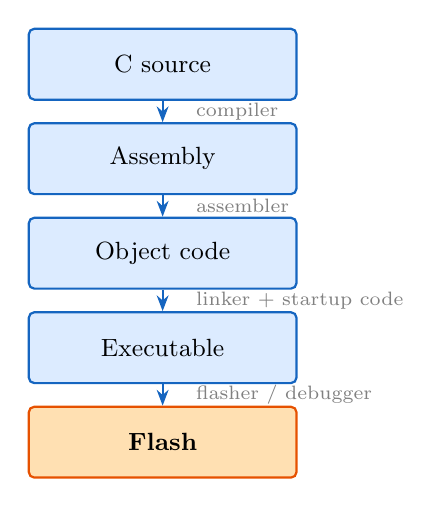
\begin{tikzpicture}[x=10mm, y=10mm]
            \node[blk,    minimum width=34mm, minimum height=9mm] (c)  at (0,2.4)  {C source};
            \node[blk,    minimum width=34mm, minimum height=9mm] (a)  at (0,1.2)  {Assembly};
            \node[blk,    minimum width=34mm, minimum height=9mm] (o)  at (0,0.0)  {Object code};
            \node[blk,    minimum width=34mm, minimum height=9mm] (e)  at (0,-1.2) {Executable};
            \node[cpublk, minimum width=34mm, minimum height=9mm] (f)  at (0,-2.4) {Flash};
            \foreach \x/\y in {c/a, a/o, o/e, e/f}{\draw[flow] (\x) -- (\y);}
            \node[lbl, anchor=west] at (0.3,1.8)  {compiler};
            \node[lbl, anchor=west] at (0.3,0.6)  {assembler};
            \node[lbl, anchor=west] at (0.3,-0.6) {linker $+$ startup code};
            \node[lbl, anchor=west] at (0.3,-1.8) {flasher / debugger};
        \end{tikzpicture}
        \end{center}
    \end{column}
    \begin{column}{.5\textwidth}
        Each step is a separate program. You can inspect each one. This
        is how you find out what your C code actually became.

        \vspace{3mm}
        \begin{block}{Why you learned assembly first}
            You will write C for the rest of this book. But when
            something goes wrong, the debugger shows you
            \alert{instructions}, not C.

            \vspace{2mm}
            Chapters 5--7 exist so this disassembly window is readable,
            not frightening.
        \end{block}

        \vspace{3mm}
        {\small The linker adds \alert{startup code}. It sets the
        stack pointer, zeroes your global variables, and calls
        \texttt{main()}, all before any line you wrote runs.}
    \end{column}
    \end{columns}
\end{frame}

\begin{frame}{C or Assembly?}
    \begin{center}
    {\small
    \striped
    \begin{tabular}{@{}l l l@{}}
        \toprule
         & \textbf{C} & \textbf{Assembly} \\
        \midrule
        Development speed & Fast & Slow \\
        Readability & Good & Poor \\
        Portability & Across ARM families & None \\
        Code size & Good, with a modern compiler & Smallest possible \\
        Hardware access & Through pointers and CMSIS & Direct \\
        Typical use & \alert{Almost everything} & Startup, ISR entry, hand-tuned DSP \\
        \bottomrule
    \end{tabular}}
    \end{center}

    \vspace{3mm}
    \begin{block}{What C gives you, and what it does not}
        C gives you the same hardware access as assembly, with far
        less bookkeeping. What it does \emph{not} give you is
        \alert{protection}. There is no runtime check to catch a bad
        pointer.
    \end{block}
\end{frame}

%===============================================================================
\section{CMSIS}
%===============================================================================

\begin{frame}{What CMSIS Is}
    \leavevmode
    {\small \textbf{C}ortex \textbf{M}icrocontroller \textbf{S}oftware
    \textbf{I}nterface \textbf{S}tandard. This is ARM's layer between
    your C code and the silicon. It works the same way across
    different chip vendors.}

    \vspace{3mm}
    \begin{columns}[T]
    \begin{column}{.48\textwidth}
        \textbf{What it gives you}
        {\small
        \begin{itemize}\itemsep1pt
            \item A \alert{struct} per peripheral, laid out on the real register
                  offsets
            \item A \alert{pointer} to each peripheral at its base address
            \item Named constants for bit fields
            \item Core functions: \texttt{\_\_enable\_irq()},
                  \texttt{NVIC\_EnableIRQ()}, \texttt{\_\_WFI()}
        \end{itemize}}
    \end{column}
    \begin{column}{.48\textwidth}
        \textbf{Why it matters}
        {\small
        \begin{itemize}\itemsep1pt
            \item The \alert{same names} across every vendor's Cortex-M
            \item Readable: \texttt{GPIOA->ODR} rather than
                  \texttt{*(volatile uint32\_t*)0x40020014}
            \item The struct layout does the address arithmetic for you
        \end{itemize}}
    \end{column}
    \end{columns}

    \vspace{2mm}
    {\small You need just one header: \texttt{\#include "stm32f446xx.h"}}
\end{frame}

\begin{frame}[plain]{The CMSIS Chain}{Silicon at the bottom, your code at the top}
    \begin{center}
    \begin{tikzpicture}[x=8mm, y=6.5mm]
    \foreach \i/\role/\what/\acc in {%
        0/{Physical hardware}/{GPIOA register block at \texttt{0x40020000}}/1,
        1/{CMSIS structure}/{\texttt{GPIO\_TypeDef} --- members at offsets \texttt{0x00}, \texttt{0x04}, \ldots}/0,
        2/{CMSIS pointer}/{\texttt{\#define GPIOA ((GPIO\_TypeDef *) 0x40020000)}}/0,
        3/{Your code}/{\texttt{GPIOA->MODER}, \texttt{GPIOA->ODR}, \texttt{GPIOA->BSRR}}/1}{
      \pgfmathsetmacro{\y}{\i*1.9}
      \ifnum\acc=1
        \node[draw=primary, fill=primary!12, thick, rounded corners=2pt,
              minimum width=76mm, minimum height=8mm, anchor=west,
              font=\scriptsize, inner sep=4pt, align=left] (L\i) at (1.4,\y) {\what};
      \else
        \node[draw=Gray, fill=Gray!8, thick, rounded corners=2pt,
              minimum width=76mm, minimum height=8mm, anchor=west,
              font=\scriptsize, inner sep=4pt, align=left] (L\i) at (1.4,\y) {\what};
      \fi
      \node[lbl, anchor=east, align=right, font=\scriptsize\bfseries] at (1.25,\y) {\role};
    }
    \foreach \a/\b/\how in {%
        0/1/{whose layout matches the hardware's register block},
        1/2/{fixed at a real address by a cast},
        2/3/{resolved by the arrow operator: base + offset}}{
      \coordinate (up\a) at ($(L\a.north west)+(0.6,0)$);
      \coordinate (dn\b) at ($(L\b.south west)+(0.6,0)$);
      \draw[flow] (dn\b) -- (up\a);
      \node[lbl, anchor=west, font=\scriptsize, text=black!60]
          at ($(up\a)!0.5!(dn\b)+(0.2,0)$) {\how};
    }
    \node[lbl, anchor=west, text=primary, align=left, font=\scriptsize] at (11.3,0) {silicon};
    \node[lbl, anchor=west, text=primary, align=left, font=\scriptsize] at (11.3,5.5) {what you type};
    \draw[decorate, decoration={brace, amplitude=4pt}, draw=Gray]
        (11.0,4.1) -- (11.0,1.35);
    \node[lbl, anchor=west, align=left, font=\scriptsize] at (11.3,2.7)
        {supplied by\\the vendor's\\header file};
    \end{tikzpicture}
    \end{center}
    \vspace{1mm}
    {\small\centering You only need to think about the top and bottom layers: the hardware exists, and your code names its registers. The two middle layers are a struct and a cast. They are written once, in a header file that you never edit.\par}
\end{frame}

\begin{frame}[fragile]{A Peripheral as a Struct}
    \begin{columns}[T]
    \begin{column}{.46\textwidth}
\begin{lstlisting}[language=C, basicstyle=\ttfamily\footnotesize]
typedef struct {
  __IO uint32_t MODER;
  __IO uint32_t OTYPER;
  __IO uint32_t OSPEEDR;
  __IO uint32_t PUPDR;
  __IO uint32_t IDR;
  __IO uint32_t ODR;
  __IO uint32_t BSRR;
  __IO uint32_t LCKR;
  __IO uint32_t AFR[2];
} GPIO_TypeDef;
\end{lstlisting}
    \end{column}
    \begin{column}{.5\textwidth}
        Each member is one \alert{32-bit register}, in hardware order.
        A \texttt{uint32\_t} is 4 bytes, so member $n$ sits at offset
        $4n$. These are exactly the offsets given in the reference
        manual.

        \vspace{2mm}
        {\small \texttt{\_\_IO} expands to \texttt{volatile}. CMSIS
        marks every register for you.}

        \vspace{2mm}
        {\small \texttt{AFR[2]} uses Chapter 3's array indexing: two
        real registers, reached as \texttt{AFR[0]} and \texttt{AFR[1]}.}
    \end{column}
    \end{columns}
\end{frame}

\begin{frame}[fragile]{From Name to Address}
    \begin{columns}[c]
    \begin{column}{.48\textwidth}
\begin{lstlisting}[language=C, basicstyle=\ttfamily\footnotesize]
#define GPIOA_BASE  0x40020000UL

#define GPIOA \
  ((GPIO_TypeDef *) GPIOA_BASE)
\end{lstlisting}

        \vspace{3mm}
        A cast turns a plain number into a pointer to the struct.
        After this, the compiler computes every register's address
        for you.

        \vspace{3mm}
        {\small \texttt{ODR} is the sixth member, so its offset is
        $5 \times 4 = 20 =$ \texttt{0x14}. This gives
        \alert{\texttt{0x40020014}}, the same address as in Chapter 1.}
    \end{column}
    \begin{column}{.48\textwidth}
        \begin{center}
        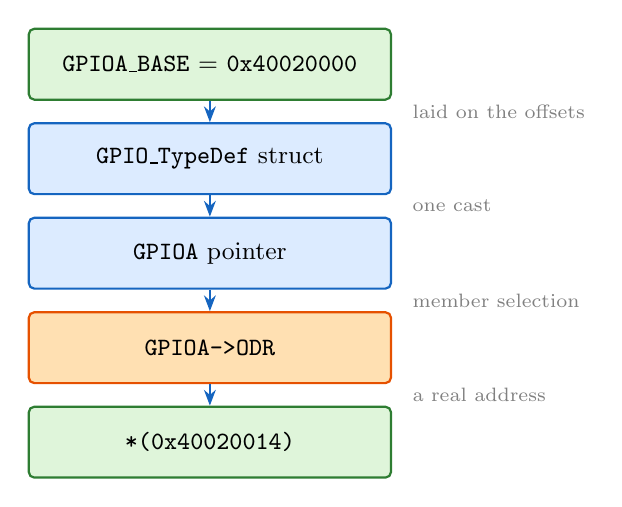
\begin{tikzpicture}[x=10mm, y=10mm]
            \node[memblk, minimum width=46mm, minimum height=9mm] (a) at (0,2.4)  {\texttt{GPIOA\_BASE} = \texttt{0x40020000}};
            \node[blk,    minimum width=46mm, minimum height=9mm] (b) at (0,1.2)  {\texttt{GPIO\_TypeDef} struct};
            \node[blk,    minimum width=46mm, minimum height=9mm] (c) at (0,0.0)  {\texttt{GPIOA} pointer};
            \node[cpublk, minimum width=46mm, minimum height=9mm] (d) at (0,-1.2) {\texttt{GPIOA->ODR}};
            \node[memblk, minimum width=46mm, minimum height=9mm] (e) at (0,-2.4) {\texttt{*(0x40020014)}};
            \foreach \x/\y in {a/b, b/c, c/d, d/e}{\draw[flow] (\x) -- (\y);}
            \node[lbl, anchor=west] at (2.45,1.8)  {laid on the offsets};
            \node[lbl, anchor=west] at (2.45,0.6)  {one cast};
            \node[lbl, anchor=west] at (2.45,-0.6) {member selection};
            \node[lbl, anchor=west] at (2.45,-1.8) {a real address};
        \end{tikzpicture}
        \end{center}
    \end{column}
    \end{columns}
\end{frame}

%===============================================================================
\section{Writing to Hardware}
%===============================================================================

\begin{frame}[fragile]{\texttt{volatile}}{Two optimisations it prevents}
    \begin{columns}[T]
    \begin{column}{.5\textwidth}
        \textbf{1. Caching a value in a register}

        \vspace{1mm}
\begin{lstlisting}[language=C, basicstyle=\ttfamily\footnotesize]
while ((*status & 1) == 0)
    ;   // waits forever without
        // volatile
\end{lstlisting}

        \vspace{2mm}
        {\small Without \texttt{volatile}, the compiler reads the
        address once, and never checks it again.}
    \end{column}
    \begin{column}{.46\textwidth}
        \textbf{2. Discarding a ``redundant'' write}

        \vspace{1mm}
\begin{lstlisting}[language=C, basicstyle=\ttfamily\footnotesize]
*reg = 1;
*reg = 0;   // without volatile the
            // first write is deleted
\end{lstlisting}

        \vspace{2mm}
        {\small Both writes matter if the address is a \alert{pulse
        output}.}
    \end{column}
    \end{columns}

    \vspace{3mm}
    \begin{block}{The rule}
        \alert{Every pointer to a hardware register must be
        \texttt{volatile}. So must every variable shared with an
        interrupt handler.}

        \vspace{1mm}
        A compiler may assume that memory only changes when the
        program changes it. For a status register updated by
        hardware, that assumption is wrong.
    \end{block}
\end{frame}

\begin{frame}[fragile]{Building a Mask: The Shift}
    \leavevmode
    Every bit idiom starts with \texttt{1U \shl\ n}. Begin with \texttt{1U}:
    only bit 0 is set. Shift it left by $n$, and the \alert{only} set
    bit is now bit $n$. This value is called a \textbf{mask}.

    \vspace{2mm}
    \begin{center}
    \begin{tikzpicture}[x=10mm, y=10mm]
    \bitrow{1.60}{bithit}{0,0,0,0,0,0,0,1}{0}{\texttt{1U}}
    \bitrow{0.10}{bithit}{0,0,1,0,0,0,0,0}{5}{\shiftl{1U}{5}}
    \draw[flow, draw=primary, thick]
        (4.34,1.33) .. controls (4.34,0.86) and (1.24,0.86) .. (1.24,0.38);
    \node[lbl, text=primary, font=\scriptsize\itshape,
          fill=white, inner sep=1.5pt] at (2.79,0.86)
         {the set bit moves 5 places left};
    \node[oplab, text width=38mm] at (5.15,0.86)
         {zeros fill in behind it, so exactly\\one bit of the mask is set.};
    \foreach \i in {0,...,7}{
        \pgfmathsetmacro{\bx}{\i*0.62}
        \pgfmathtruncatemacro{\bn}{7-\i}
        \node[font=\tiny, text=black!45] at (\bx,2.08) {\bn};
    }
    \node[rowlab, font=\tiny, text=black!45] at (-0.55,2.08) {bit};
    \end{tikzpicture}
    \end{center}

    \vspace{2mm}
    \begin{block}{The shift count \emph{is} the bit number}
        \texttt{1U \shl\ 5} selects bit 5, not bit 6. Writing the pin
        number directly in the shift keeps the code readable, and easy
        to change for a different pin.
    \end{block}
\end{frame}

\begin{frame}{Why the \texttt{U} Suffix}
    \leavevmode
    A plain \texttt{1} is signed. Its top bit is the sign bit. C treats
    signed and unsigned shifts differently, and this difference
    matters exactly here.

    \vspace{2mm}
    \begin{center}
    \begin{tikzpicture}[x=10mm, y=10mm]
    \bitrow{1.95}{bithit}{1,0,0,1,0,1,0,0}{7}{start}
    \bitrow{0.85}{bitmask}{0,1,0,0,1,0,1,0}{7}{\shiftx{unsigned}{\shr}{1}}
    \bitrow{-0.15}{bithit}{1,1,0,0,1,0,1,0}{7}{\shiftx{signed}{\shr}{1}}
    \node[oplab, text width=40mm] at (5.15,0.85)
         {a \textbf{0} is shifted in: the value\\simply halves.};
    \node[oplab, text width=40mm] at (5.15,-0.15)
         {the \textbf{sign bit is copied}: a negative\\value stays negative.};
    \draw[draw=primary, thick, -{Stealth[length=1.6mm]}]
        (0,-0.78) -- (0,-0.45);
    \node[lbl, anchor=north, text=primary] at (0,-0.83) {bit 7, the sign bit};
    \foreach \i in {0,...,7}{
        \pgfmathsetmacro{\bx}{\i*0.62}
        \pgfmathtruncatemacro{\bn}{7-\i}
        \node[font=\tiny, text=black!45] at (\bx,2.43) {\bn};
    }
    \node[rowlab, font=\tiny, text=black!45] at (-0.55,2.43) {bit};
    \end{tikzpicture}
    \end{center}

    \vspace{1mm}
    {\small \texttt{1 \shl\ 31} is \alert{undefined behaviour} on a
    32-bit \texttt{int}. \texttt{1U \shl\ 31} is fully defined, and gives
    \texttt{0x80000000}. A register is 32 switches, not a signed
    number. Always write \texttt{U}.}
\end{frame}

\begin{frame}{Setting a Bit: \texttt{|=}}
    \leavevmode
    \begin{center}
    \begin{tikzpicture}[x=10mm, y=10mm]
    \bitrow{1.30}{bithit}{0,0,0,1,0,1,0,0}{5}{original}
    \bitrow{0.55}{bitmask}{0,0,1,0,0,0,0,0}{5}{\shiftx{|= (1U}{\shl}{5)}}
    \draw[Gray, thick] (-0.36,0.12) -- (4.70,0.12);
    \bitrow{-0.35}{bithit}{0,0,1,1,0,1,0,0}{5}{result}
    \draw[draw=primary, thick, -{Stealth[length=1.6mm]}] (1.24,-0.95) -- (1.24,-0.62);
    \node[lbl, anchor=north, text=primary] at (1.24,-1.0) {bit 5};
    \node[oplab, text width=44mm] at (5.0,0.48) {OR with 1 forces a bit to 1;\\OR with 0 leaves it alone.};
    \foreach \i in {0,...,7}{
        \pgfmathsetmacro{\bx}{\i*0.62}
        \pgfmathtruncatemacro{\bn}{7-\i}
        \node[font=\tiny, text=black!45] at (\bx,1.78) {\bn};
    }
    \node[rowlab, font=\tiny, text=black!45] at (-0.55,1.78) {bit};
    \end{tikzpicture}
    \end{center}
    \vspace{2mm}
    {\small\centering \texttt{GPIOA->ODR |= (1U \shl\ 5);} --- only the masked bit changes; every other bit is OR-ed with 0 and passes through untouched.\par}
\end{frame}

\begin{frame}{Clearing a Bit: \texttt{\&=} with an Inverted Mask}
    \leavevmode
    \begin{center}
    \begin{tikzpicture}[x=10mm, y=10mm]
    \bitrow{1.30}{bithit}{0,0,1,1,0,1,0,0}{5}{original}
    \bitrow{0.55}{bitmask}{1,1,0,1,1,1,1,1}{5}{\shiftx{\&= \textasciitilde{}(1U}{\shl}{5)}}
    \draw[Gray, thick] (-0.36,0.12) -- (4.70,0.12);
    \bitrow{-0.35}{bithit}{0,0,0,1,0,1,0,0}{5}{result}
    \draw[draw=primary, thick, -{Stealth[length=1.6mm]}] (1.24,-0.95) -- (1.24,-0.62);
    \node[lbl, anchor=north, text=primary] at (1.24,-1.0) {bit 5};
    \node[oplab, text width=44mm] at (5.0,0.48) {AND with 0 forces a bit to 0;\\AND with 1 leaves it alone.};
    \foreach \i in {0,...,7}{
        \pgfmathsetmacro{\bx}{\i*0.62}
        \pgfmathtruncatemacro{\bn}{7-\i}
        \node[font=\tiny, text=black!45] at (\bx,1.78) {\bn};
    }
    \node[rowlab, font=\tiny, text=black!45] at (-0.55,1.78) {bit};
    \end{tikzpicture}
    \end{center}
    \vspace{2mm}
    {\small\centering \texttt{GPIOA->ODR \&= \textasciitilde(1U \shl\ 5);} --- the tilde makes every bit except bit 5 a 1, so only bit 5 is forced low. The compiler emits \texttt{BIC}.\par}
\end{frame}

\begin{frame}{Toggling a Bit: \texttt{\^{}=}}
    \leavevmode
    \begin{center}
    \begin{tikzpicture}[x=10mm, y=10mm]
    \bitrow{1.30}{bithit}{0,0,1,1,0,1,0,0}{5}{original}
    \bitrow{0.55}{bitmask}{0,0,1,0,0,0,0,0}{5}{\shiftx{\textasciicircum{}= (1U}{\shl}{5)}}
    \draw[Gray, thick] (-0.36,0.12) -- (4.70,0.12);
    \bitrow{-0.35}{bithit}{0,0,0,1,0,1,0,0}{5}{result}
    \draw[draw=primary, thick, -{Stealth[length=1.6mm]}] (1.24,-0.95) -- (1.24,-0.62);
    \node[lbl, anchor=north, text=primary] at (1.24,-1.0) {bit 5};
    \node[oplab, text width=44mm] at (5.0,0.48) {XOR with 1 inverts a bit;\\XOR with 0 preserves it.};
    \foreach \i in {0,...,7}{
        \pgfmathsetmacro{\bx}{\i*0.62}
        \pgfmathtruncatemacro{\bn}{7-\i}
        \node[font=\tiny, text=black!45] at (\bx,1.78) {\bn};
    }
    \node[rowlab, font=\tiny, text=black!45] at (-0.55,1.78) {bit};
    \end{tikzpicture}
    \end{center}
    \vspace{2mm}
    {\small\centering \texttt{GPIOA->ODR \^{}= (1U \shl\ 5);} --- the same statement run twice returns the register to its starting value, which is why one line suffices to blink an LED.\par}
\end{frame}

\begin{frame}{Multi-Bit Fields: Clear, Then Set}
    \leavevmode
    OR alone cannot clear a bit. Say \texttt{MODER} bits 11:10 read
    \texttt{11}, and you OR in \texttt{01}. The result is still
    \texttt{11}. You must clear the field first, before setting it.

    \vspace{2mm}
    \begin{center}
    \begin{tikzpicture}[x=10mm, y=8mm]
    \bitfieldrow{2.10}{bithit}{0,0,0,0,1,1,0,0}{2}{original}
    \bitfieldrow{1.35}{bitmask}{1,1,1,1,0,0,1,1}{2}{\shiftx{\&= \textasciitilde{}(3U}{\shl}{10)}}
    \draw[Gray, thick] (-0.36,0.95) -- (4.70,0.95);
    \bitfieldrow{0.55}{bithit}{0,0,0,0,0,0,0,0}{2}{cleared}
    \bitfieldrow{-0.35}{bitmask}{0,0,0,0,0,1,0,0}{2}{\shiftx{|= (1U}{\shl}{10)}}
    \draw[Gray, thick] (-0.36,-0.78) -- (4.70,-0.78);
    \bitfieldrow{-1.20}{bithit}{0,0,0,0,0,1,0,0}{2}{result}
    \draw[draw=primary, thick, decorate,
          decoration={brace, amplitude=3pt, mirror}] (2.21,-1.52) -- (3.37,-1.52);
    \node[lbl, anchor=north, text=primary] at (2.79,-1.62) {bits 11:10};
    \node[oplab, text width=46mm] at (5.0,1.35) {OR alone cannot clear a bit, so a\\multi-bit field must be zeroed first\ldots};
    \node[oplab, text width=46mm] at (5.0,-0.35) {\ldots{}and only then written with the\\value you want.};
    \foreach \i in {0,...,7}{
        \pgfmathsetmacro{\bx}{\i*0.62}
        \pgfmathtruncatemacro{\bn}{15-\i}
        \node[font=\tiny, text=black!45] at (\bx,2.58) {\bn};
    }
    \node[rowlab, font=\tiny, text=black!45] at (-0.55,2.58) {bit};
    \end{tikzpicture}
    \end{center}
\end{frame}

\begin{frame}{The Four Bit Operations}
    \begin{center}
    {\small
    \striped
    \begin{tabular}{@{}l l l@{}}
        \toprule
        \textbf{Goal} & \textbf{In C} & \textbf{Compiles to} \\
        \midrule
        Set bit $n$    & \texttt{REG |= (1U \shl\ n);}      & \texttt{ORR} \\
        Clear bit $n$  & \texttt{REG \&= \textasciitilde(1U \shl\ n);} & \texttt{BIC} \\
        Toggle bit $n$ & \texttt{REG \^{}= (1U \shl\ n);}   & \texttt{EOR} \\
        Test bit $n$   & \texttt{if (REG \& (1U \shl\ n))}  & \texttt{TST} \\
        \bottomrule
    \end{tabular}}
    \end{center}

    \vspace{3mm}
    \begin{block}{Read--modify--write}
        A peripheral register holds settings for \alert{many} pins.
        You must keep the bits you are not changing. \texttt{|=} and
        \texttt{\&=} do this automatically. A plain \texttt{=} would
        wipe out every other setting.
    \end{block}

    \vspace{2mm}
    {\small A multi-bit field needs a \alert{mask}: first clear it
    with \texttt{\&= \textasciitilde(3U \shl\ pos)}, then set it with
    \texttt{|= (value \shl\ pos)}. The mask is always ``all ones for this
    field.''}
\end{frame}

\begin{frame}[fragile]{A Complete Bare-Metal Program}
    \begin{columns}[T]
    \begin{column}{.56\textwidth}
\begin{lstlisting}[language=C, basicstyle=\ttfamily\footnotesize]
#include "stm32f446xx.h"

int main(void)
{
  // 1. Enable the clock for GPIOA
  RCC->AHB1ENR |= (1U << 0);

  // 2. Set PA5 as an output
  GPIOA->MODER &= ~(3U << (5*2));
  GPIOA->MODER |=  (1U << (5*2));

  // 3. Toggle PA5 forever
  while (1) {
    GPIOA->ODR ^= (1U << 5);
    for (volatile int i = 0;
         i < 100000; i++);
  }
}
\end{lstlisting}
    \end{column}
    \begin{column}{.4\textwidth}
        \textbf{Every idea in this chapter}
        {\small
        \begin{itemize}\itemsep1pt
            \item Struct-based register access
            \item Bit masking and shifting
            \item Read--modify--write
            \item Clock enable, then configure
        \end{itemize}}

        \vspace{2mm}
        {\small \textbf{Why \texttt{5*2}?} \texttt{MODER} gives each
        pin \alert{two} bits, so pin 5's bits start at position 10.}

        \vspace{2mm}
        {\small \textbf{Why \texttt{volatile} on \texttt{i}?} Without
        it, the optimiser deletes the whole delay loop.}
    \end{column}
    \end{columns}
\end{frame}

\begin{frame}{The Clock Must Come First}
    \begin{columns}[T]
    \begin{column}{.5\textwidth}
        {\ttfamily\normalsize RCC->AHB1ENR |= (1U \shl\ 0);}

        \vspace{3mm}
        \begin{itemize}
            \item Every peripheral starts with its \alert{clock
                  disabled}, to save power.
            \item A peripheral with no clock does not respond to
                  writes. They are simply \alert{lost}.
            \item \texttt{RCC} is the Reset and Clock Control
                  peripheral. GPIOA is bit 0 of \texttt{AHB1ENR}.
        \end{itemize}
    \end{column}
    \begin{column}{.46\textwidth}
        \begin{block}{The classic first bug}
            You write the GPIO configuration. The code compiles and
            runs. But \alert{nothing happens}. No fault, no error: the
            writes went nowhere, because the clock was off.

            \vspace{2mm}
            \alert{Enable the clock first.} Always.
        \end{block}
    \end{column}
    \end{columns}
\end{frame}

\begin{frame}{Summary}
	\begin{columns}[c]
		\begin{column}{.62\textwidth}
			\begin{center}
				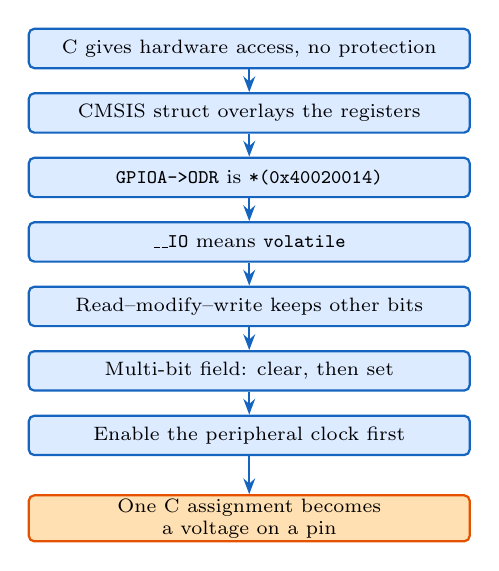
\begin{tikzpicture}[x=10mm, y=7.8mm]
					\node[blk, minimum width=56mm, minimum height=5.0mm, inner sep=1.2pt, font=\scriptsize] (n0) at (0,0.00) {C gives hardware access, no protection};
					\node[blk, minimum width=56mm, minimum height=5.0mm, inner sep=1.2pt, font=\scriptsize] (n1) at (0,-1.05) {CMSIS struct overlays the registers};
					\node[blk, minimum width=56mm, minimum height=5.0mm, inner sep=1.2pt, font=\scriptsize] (n2) at (0,-2.10) {\texttt{GPIOA->ODR} is \texttt{*(0x40020014)}};
					\node[blk, minimum width=56mm, minimum height=5.0mm, inner sep=1.2pt, font=\scriptsize] (n3) at (0,-3.15) {\texttt{\_\_IO} means \texttt{volatile}};
					\node[blk, minimum width=56mm, minimum height=5.0mm, inner sep=1.2pt, font=\scriptsize] (n4) at (0,-4.20) {Read--modify--write keeps other bits};
					\node[blk, minimum width=56mm, minimum height=5.0mm, inner sep=1.2pt, font=\scriptsize] (n5) at (0,-5.25) {Multi-bit field: clear, then set};
					\node[blk, minimum width=56mm, minimum height=5.0mm, inner sep=1.2pt, font=\scriptsize] (n6) at (0,-6.30) {Enable the peripheral clock first};
					\node[cpublk, minimum width=56mm, minimum height=5.0mm, inner sep=1.2pt, font=\scriptsize, align=center] (n7) at (0,-7.65) {One C assignment becomes\\a voltage on a pin};
					\foreach \a/\b in {0/1,1/2,2/3,3/4,4/5,5/6,6/7}{\draw[flow] (n\a) -- (n\b);}
				\end{tikzpicture}
			\end{center}
		\end{column}
		\begin{column}{.34\textwidth}
			{\scriptsize
				\textbf{Terminology covered}\\[1mm]
				\begin{itemize}
					\item CMSIS, device header
					\item Struct overlay
					\item \texttt{volatile}, \texttt{\_\_IO}
					\item Set, clear, toggle, test
					\item Peripheral clock enable
				\end{itemize}
				\vspace{3mm}
				\textbf{Next: Chapter 5}\\[1mm]
				\emph{ARM Assembly Fundamentals}\\[1mm]
				We read what this C compiles to.}
		\end{column}
	\end{columns}
\end{frame}

\end{document}

